\section{Introduction}
\label{ch:intro}

The Coronavirus disease (COVID-19) was first characterized by the World Health Organisation as pandemic on 11th March 2020 \cite{whodeclare20}. The outbreak has affected almost every aspect of human life throughout 2020, and is expected to continue for much of 2021. 

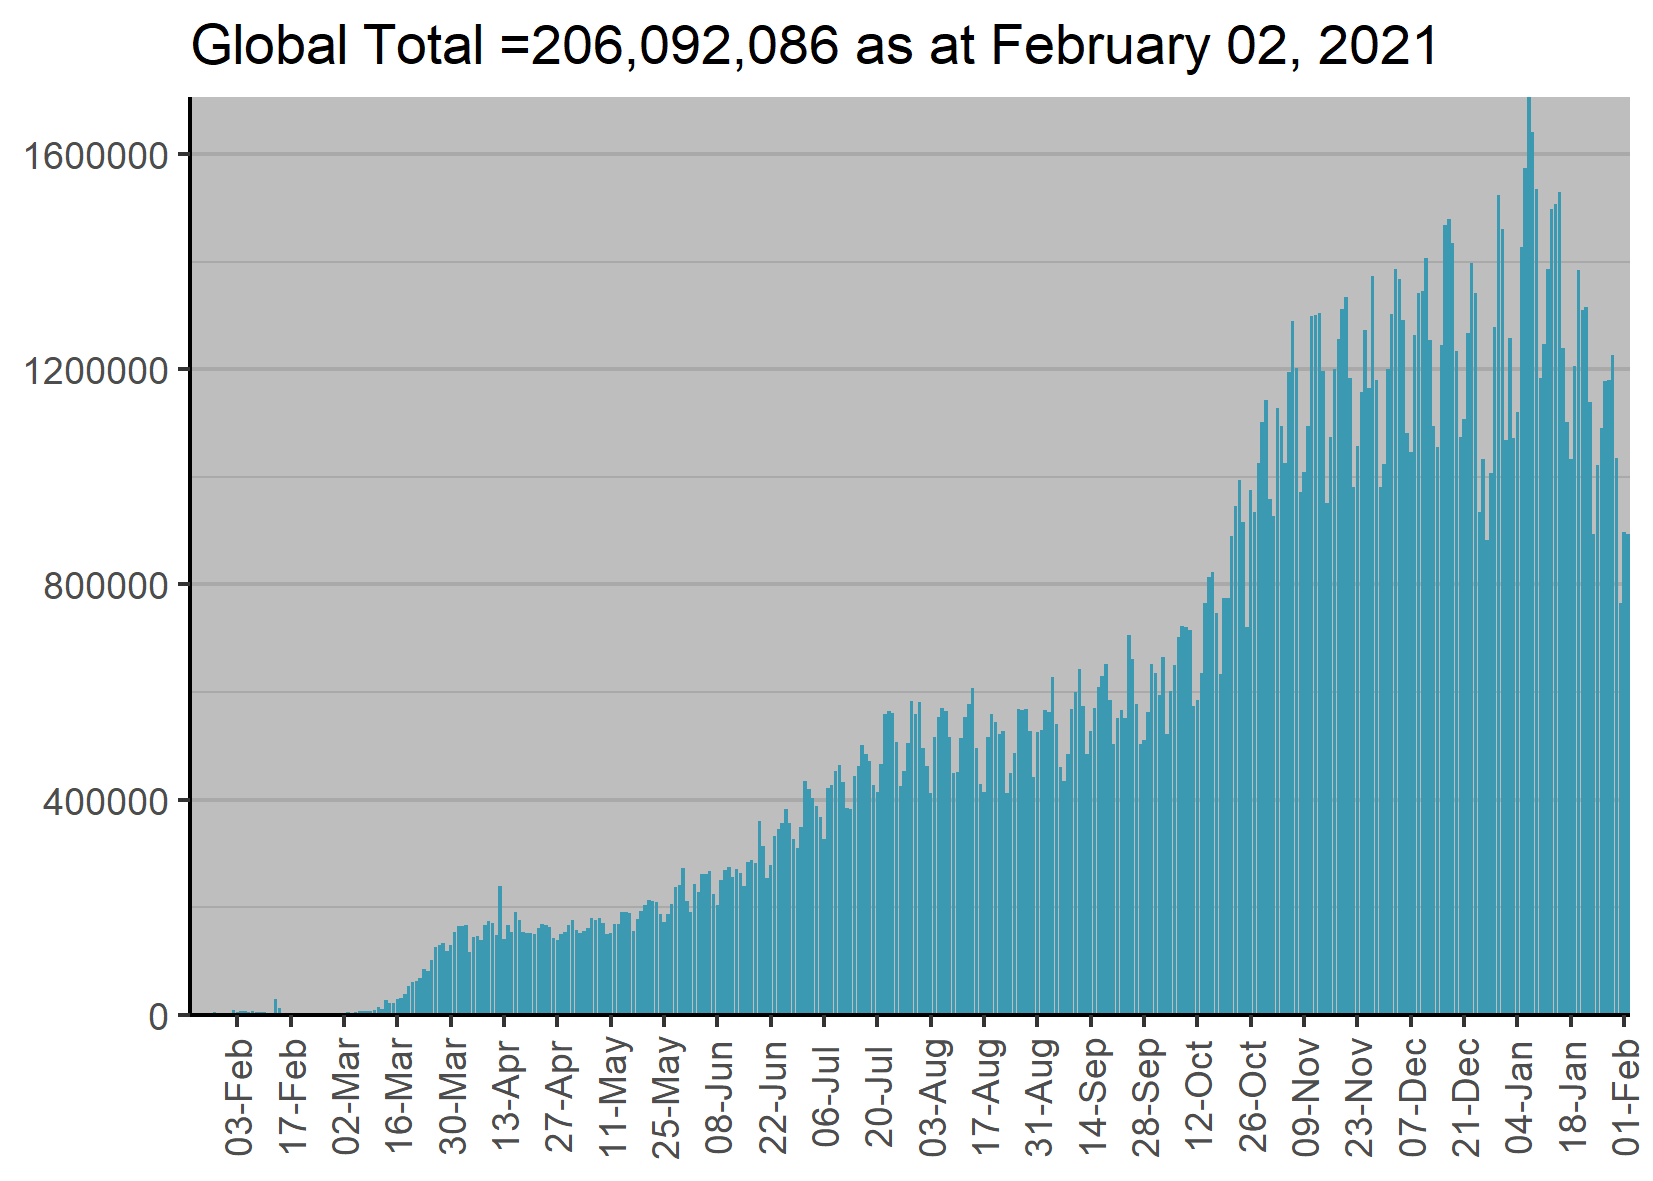
\includegraphics[width=0.9\textwidth]{WorldTotal-xn.png}

We can map the cumulative number of cases per 100,000 population for each country to see the varying severity of disease spread. 

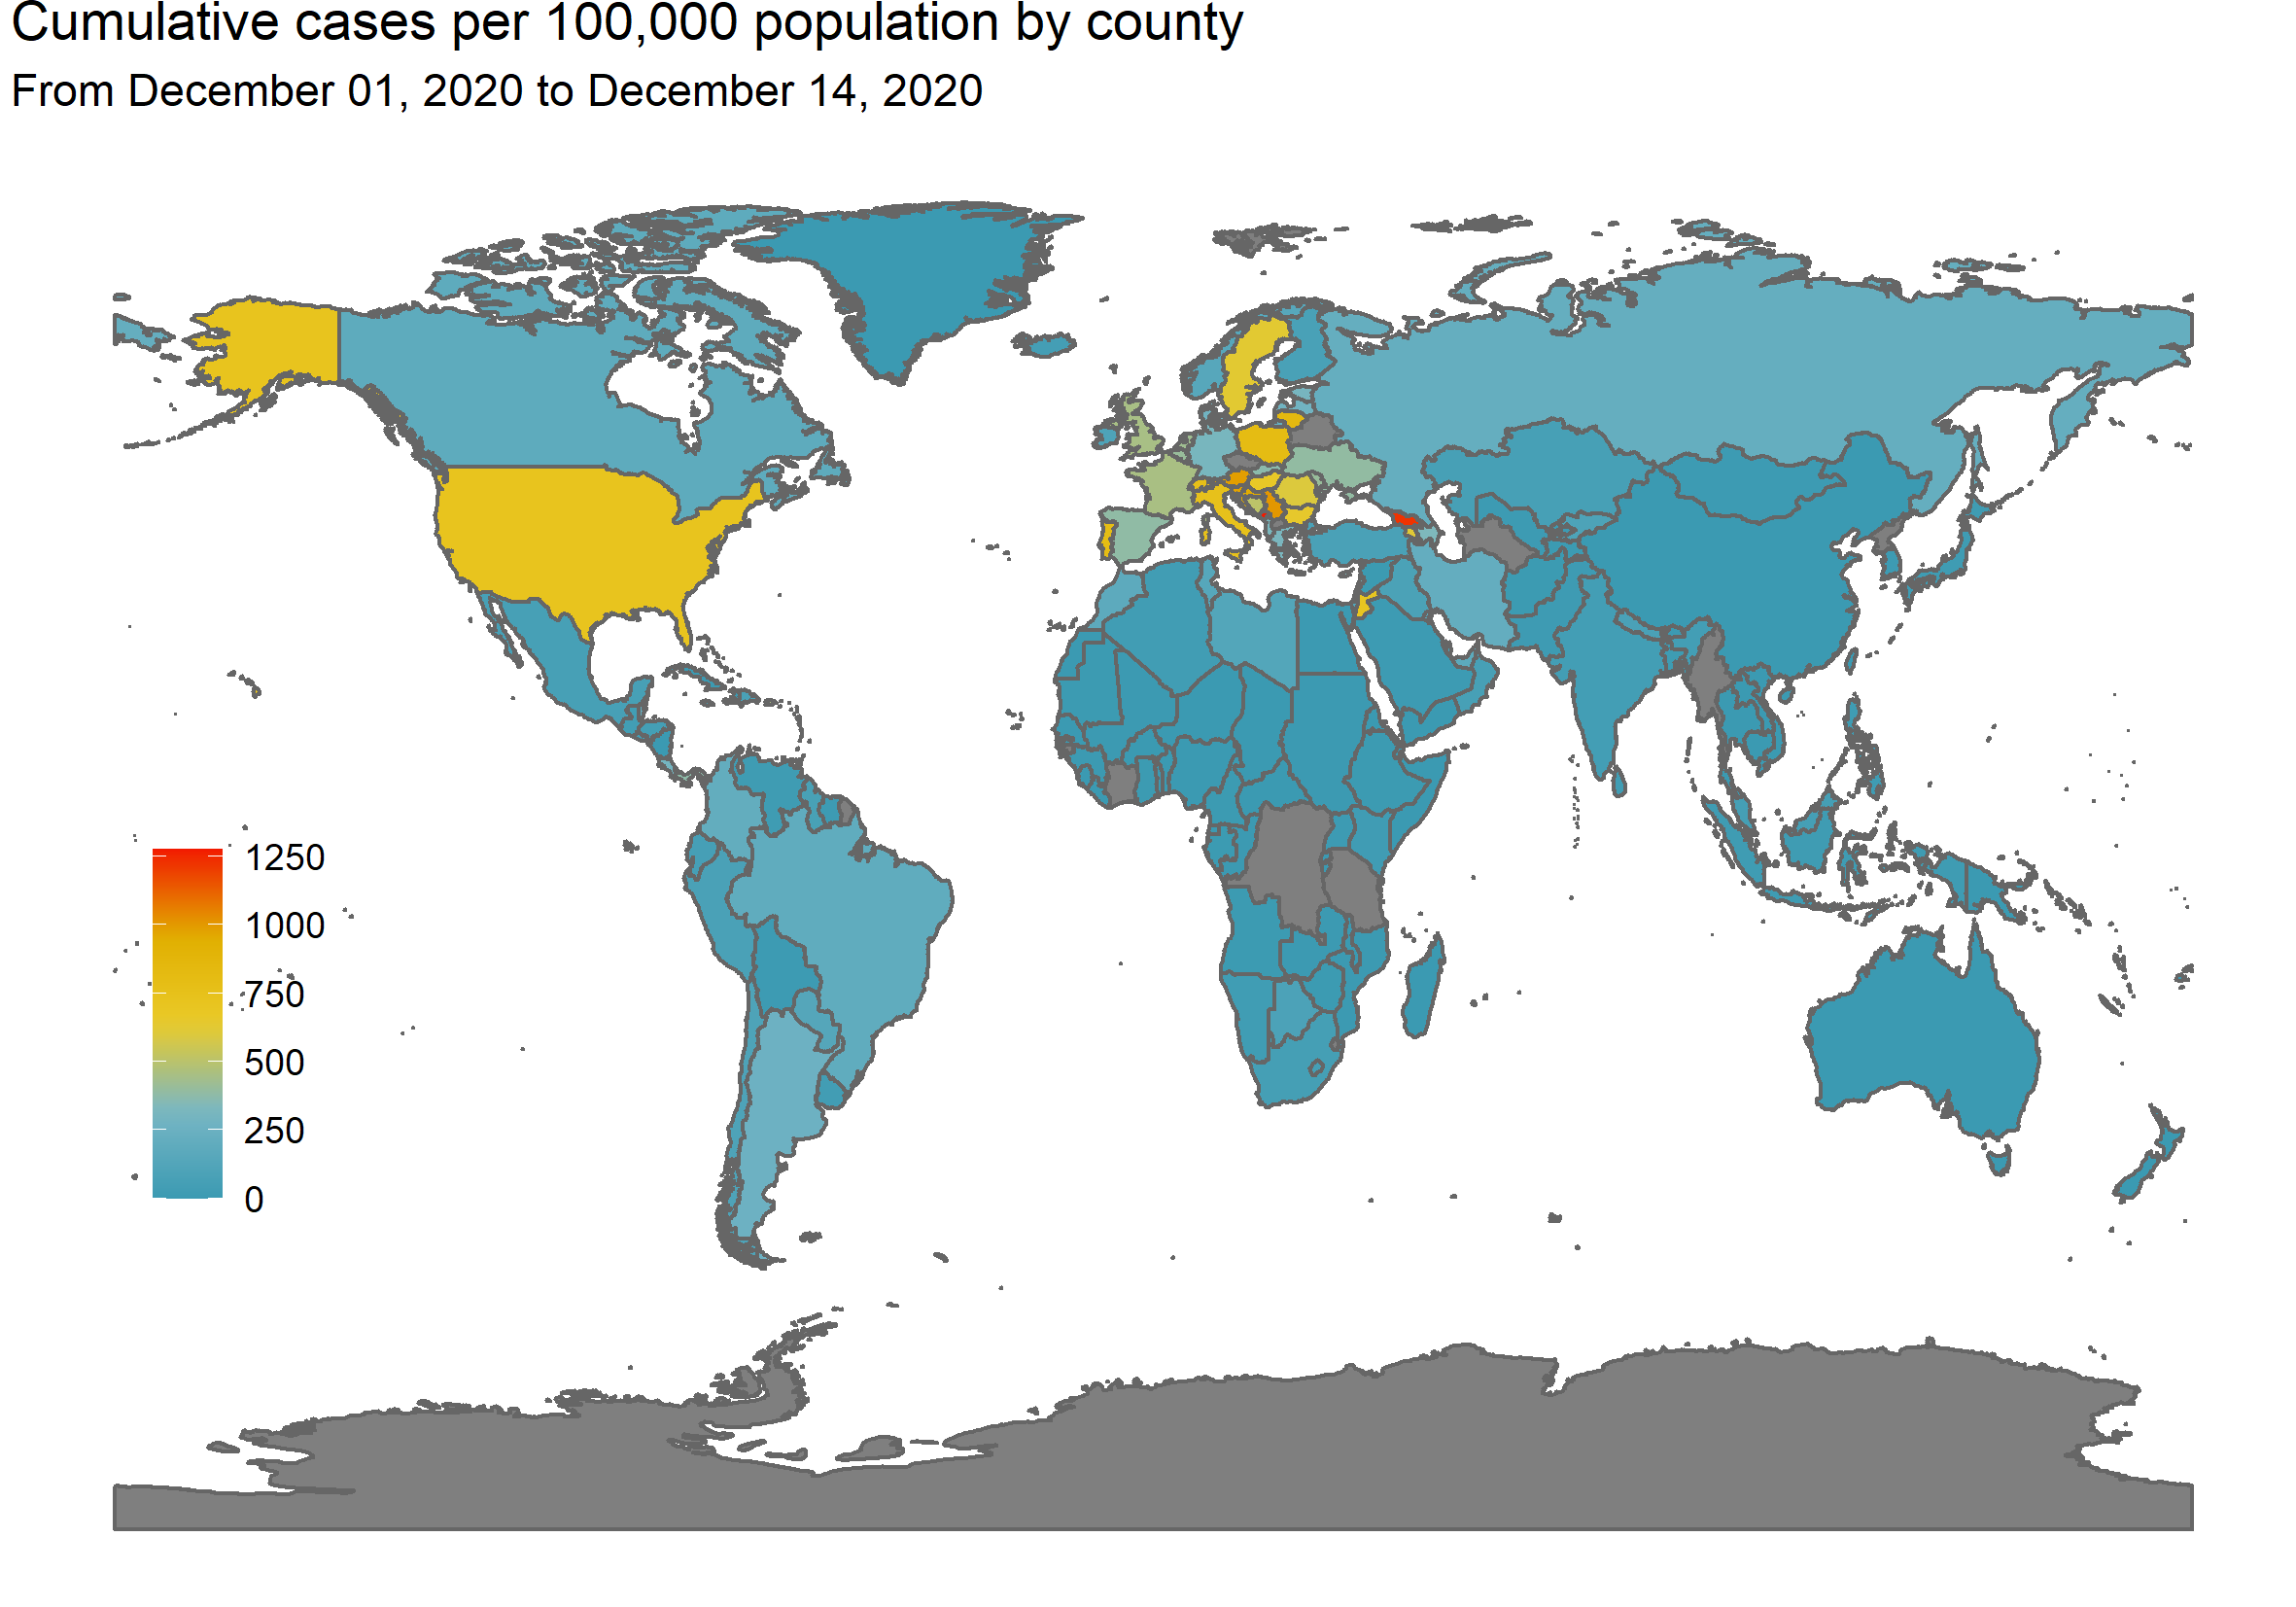
\includegraphics[width=0.9\textwidth]{world-blank.png}

Europe is experiencing an especially high number of cases, proportionally, as well as the US.

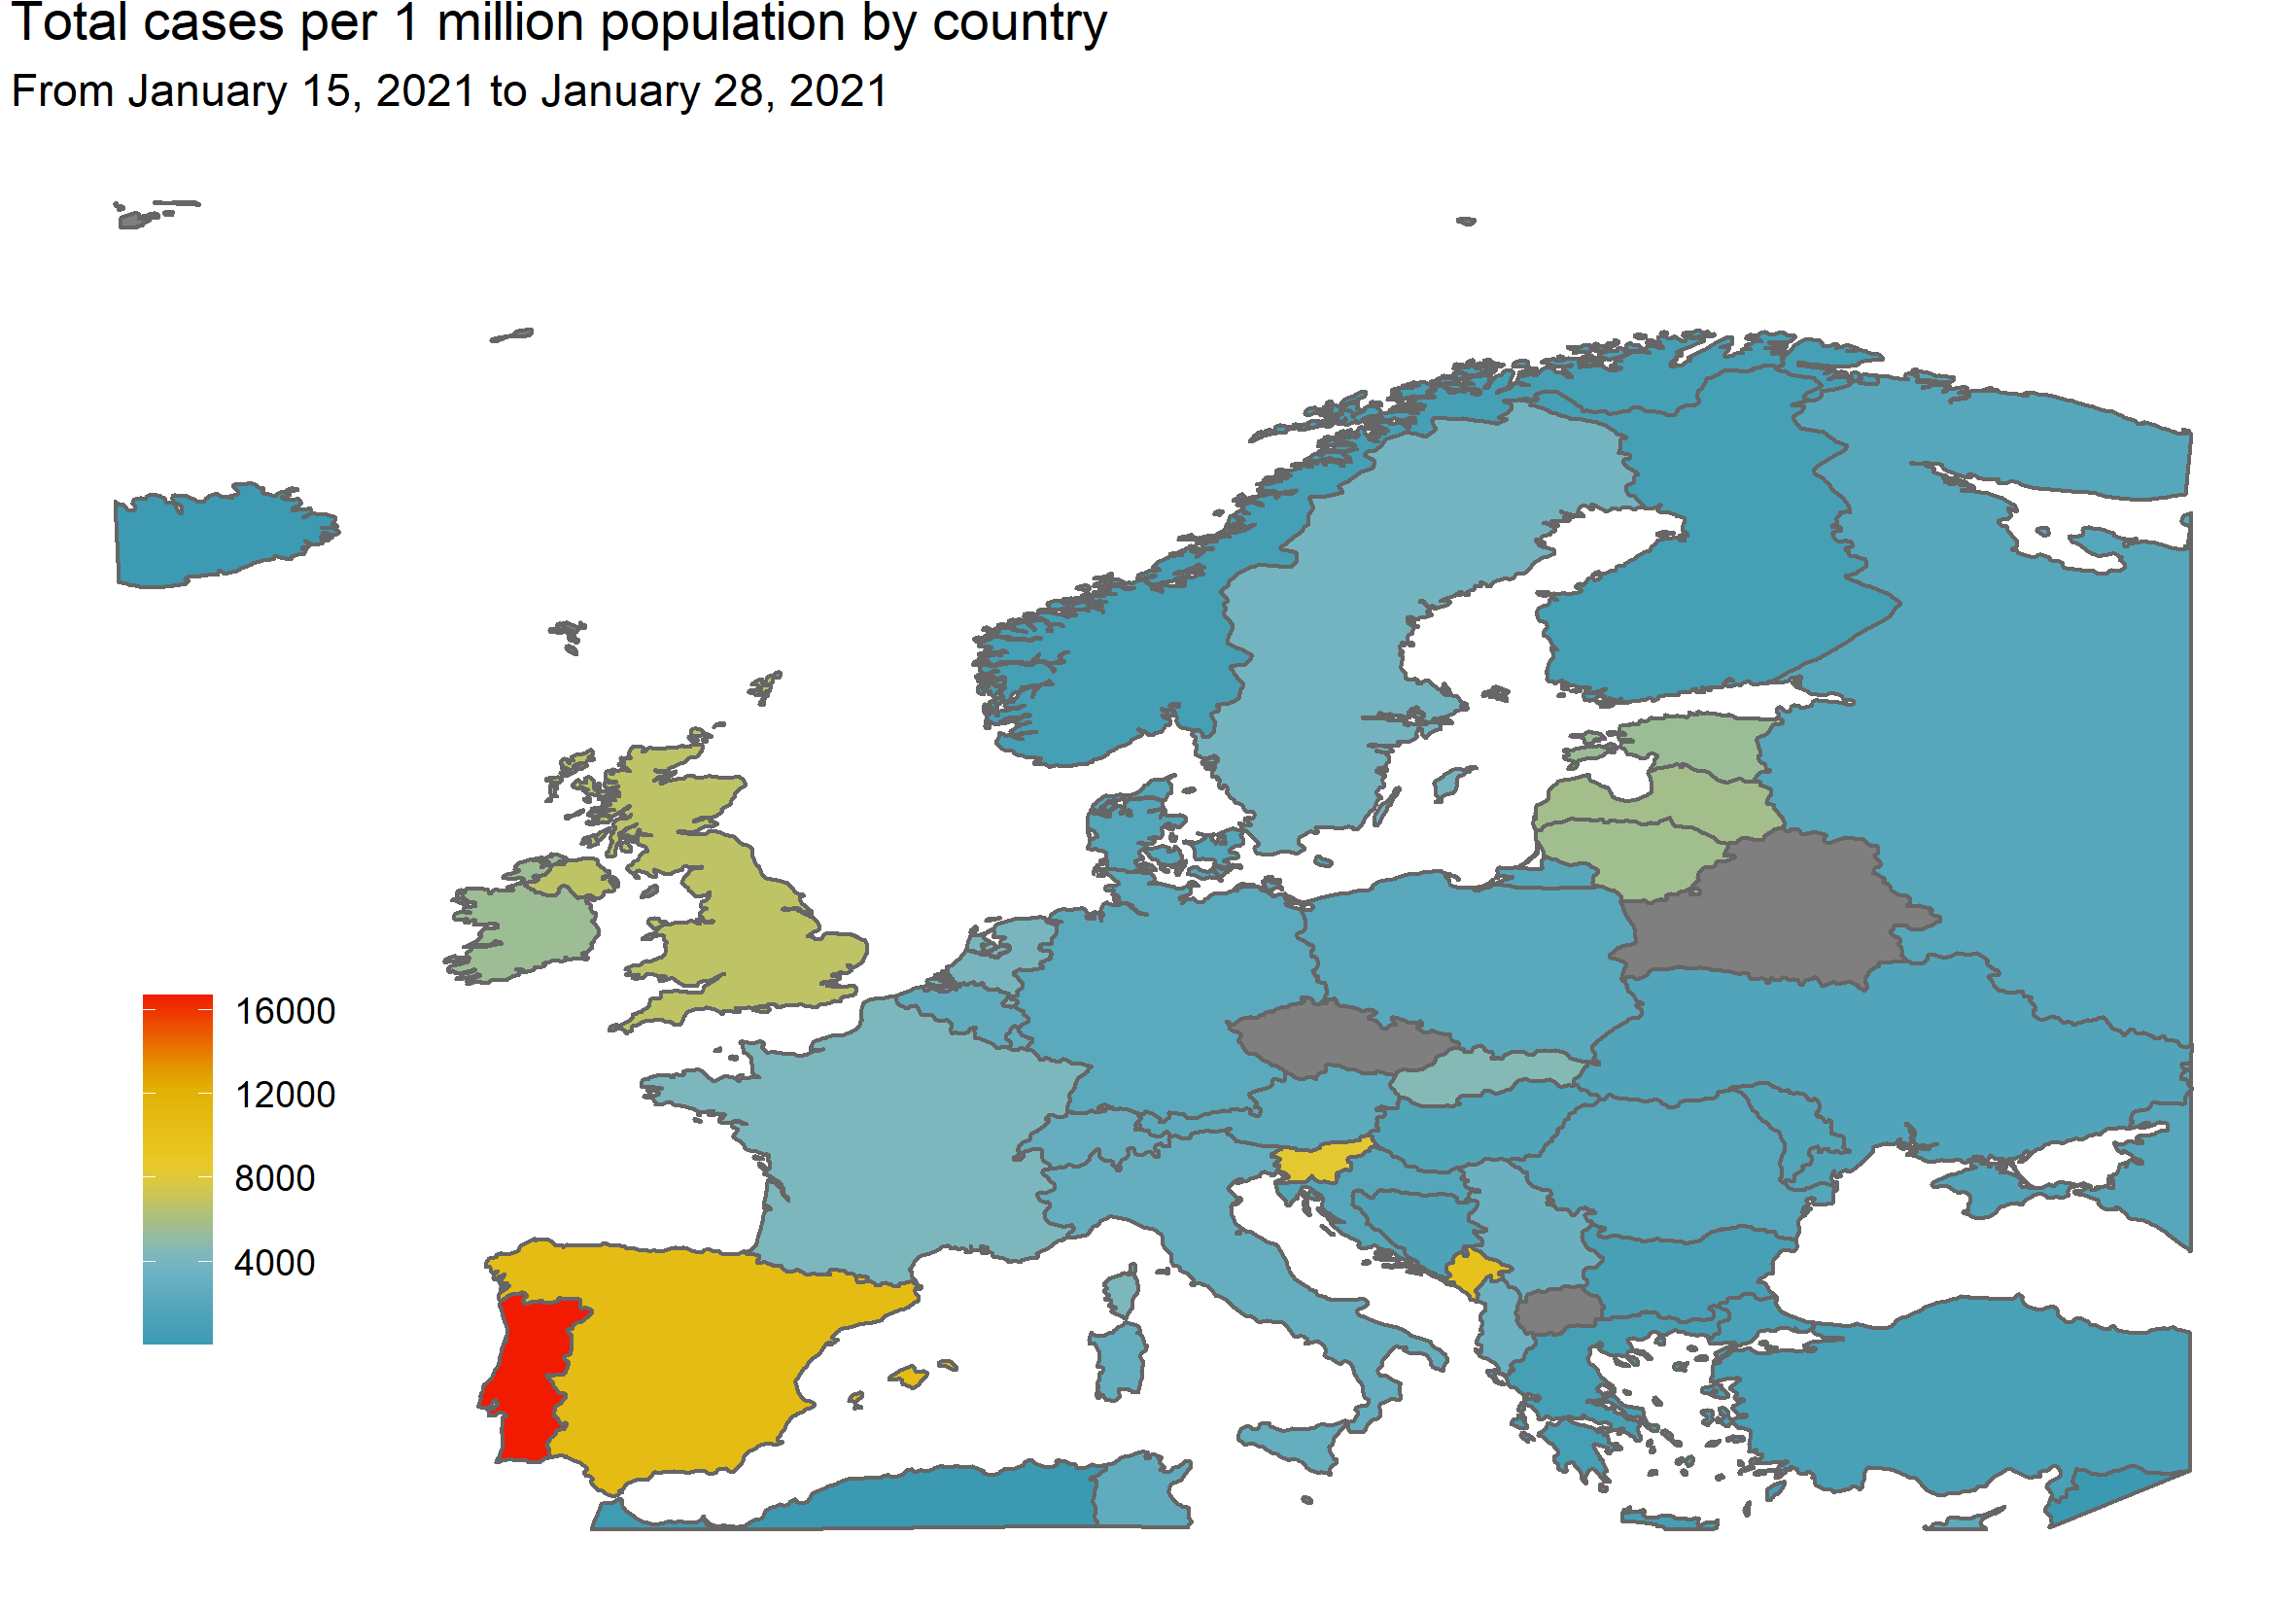
\includegraphics[width=0.9\textwidth]{world-europe.png}

More locally, we see that Ireland also has a clear variation in concentration of cases to date, with Donegal and much of Leinster experiencing sometimes twice as many cases per 100,000 population as the rest of the country.

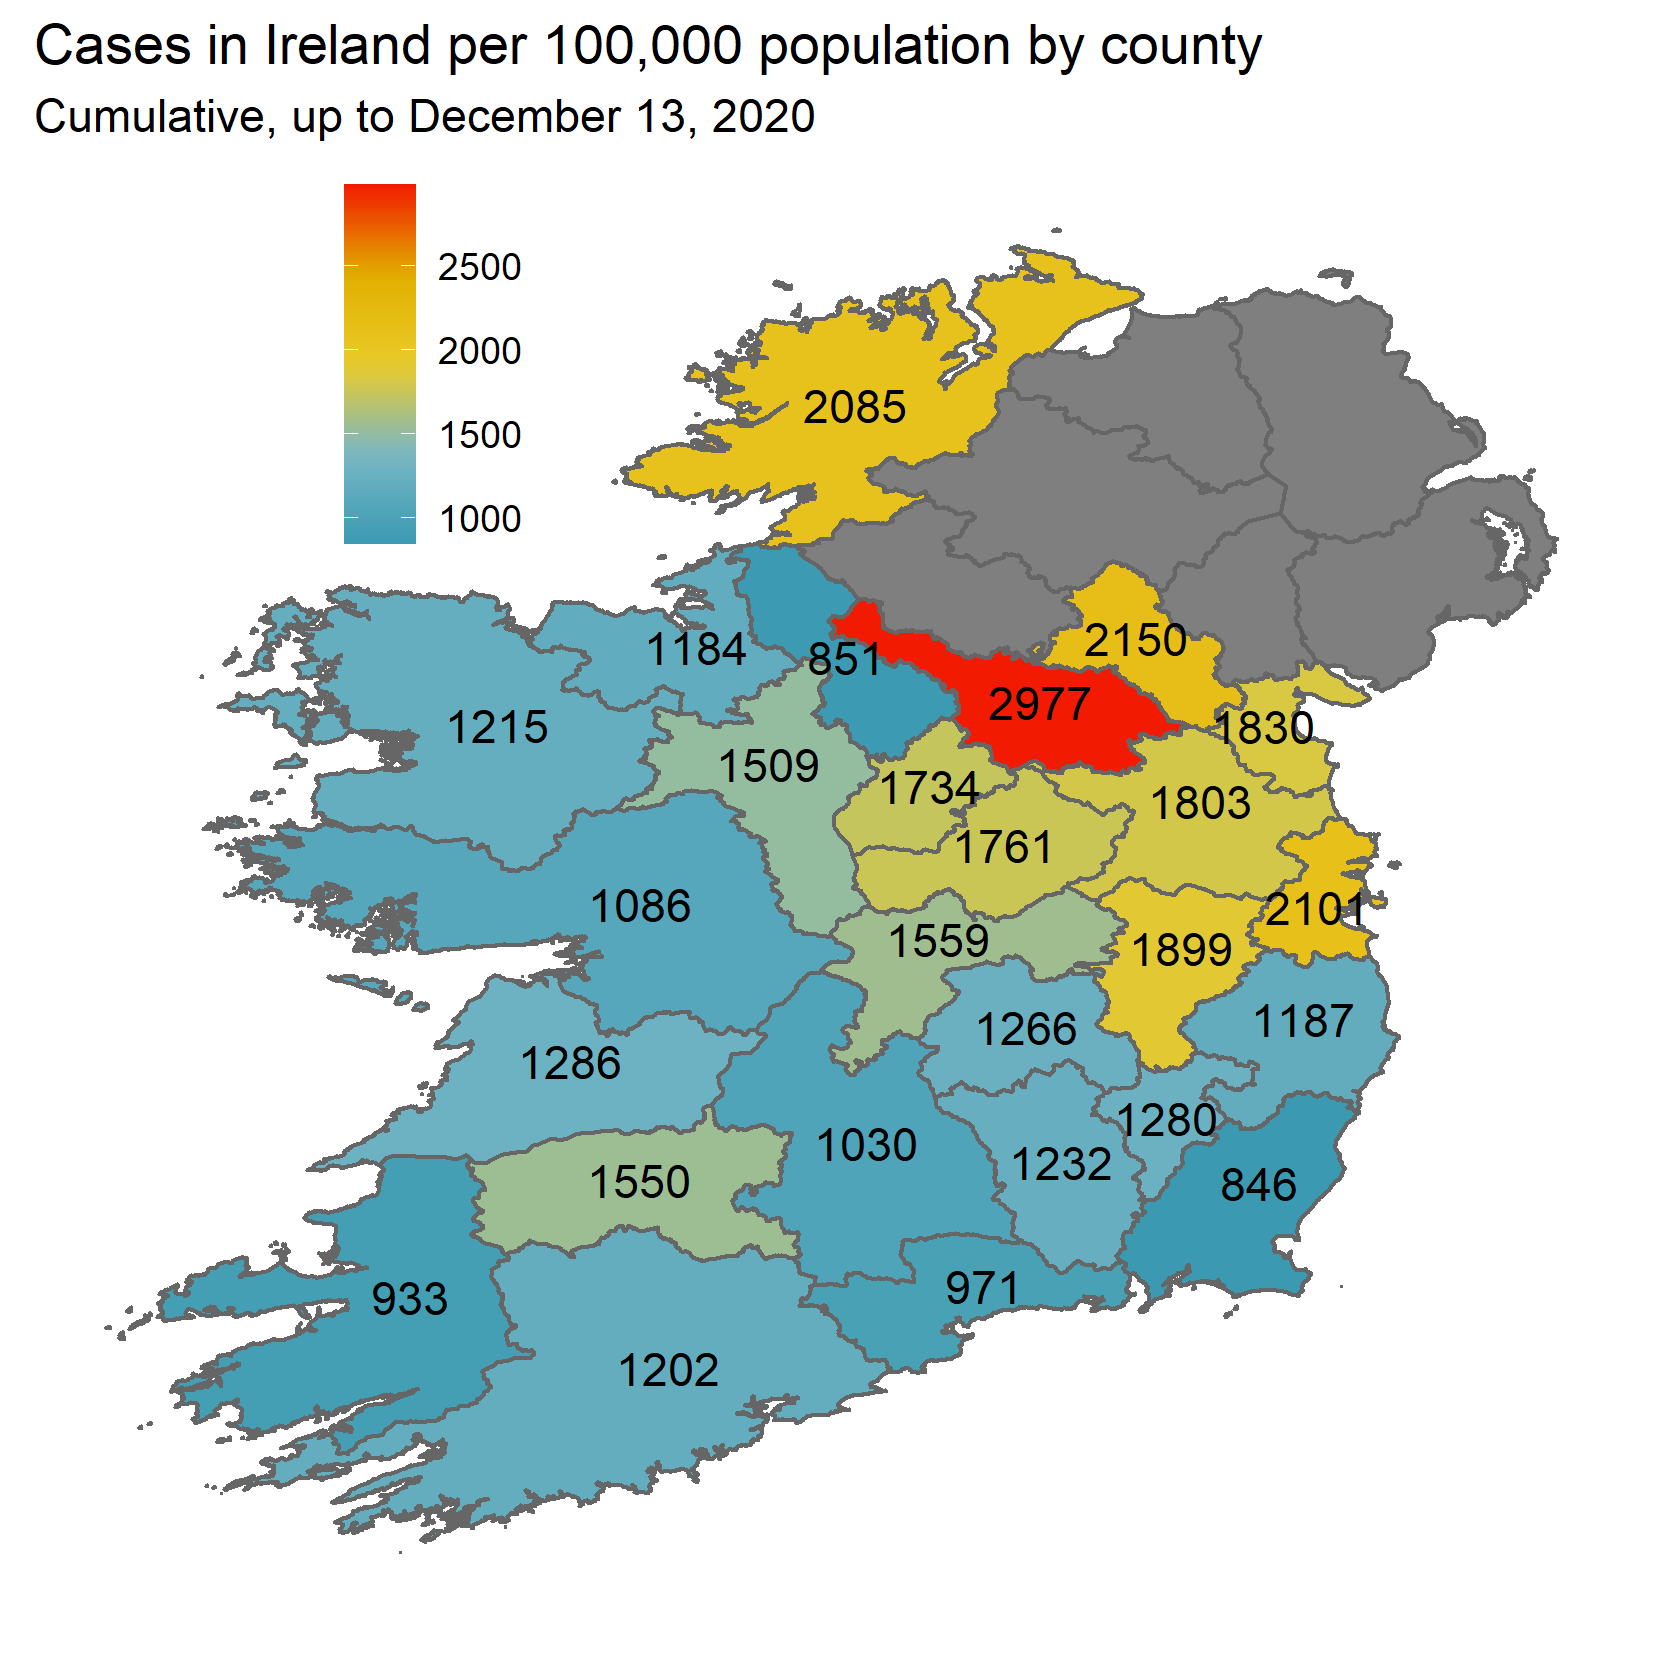
\includegraphics[width=0.9\textwidth]{county-rep.png}

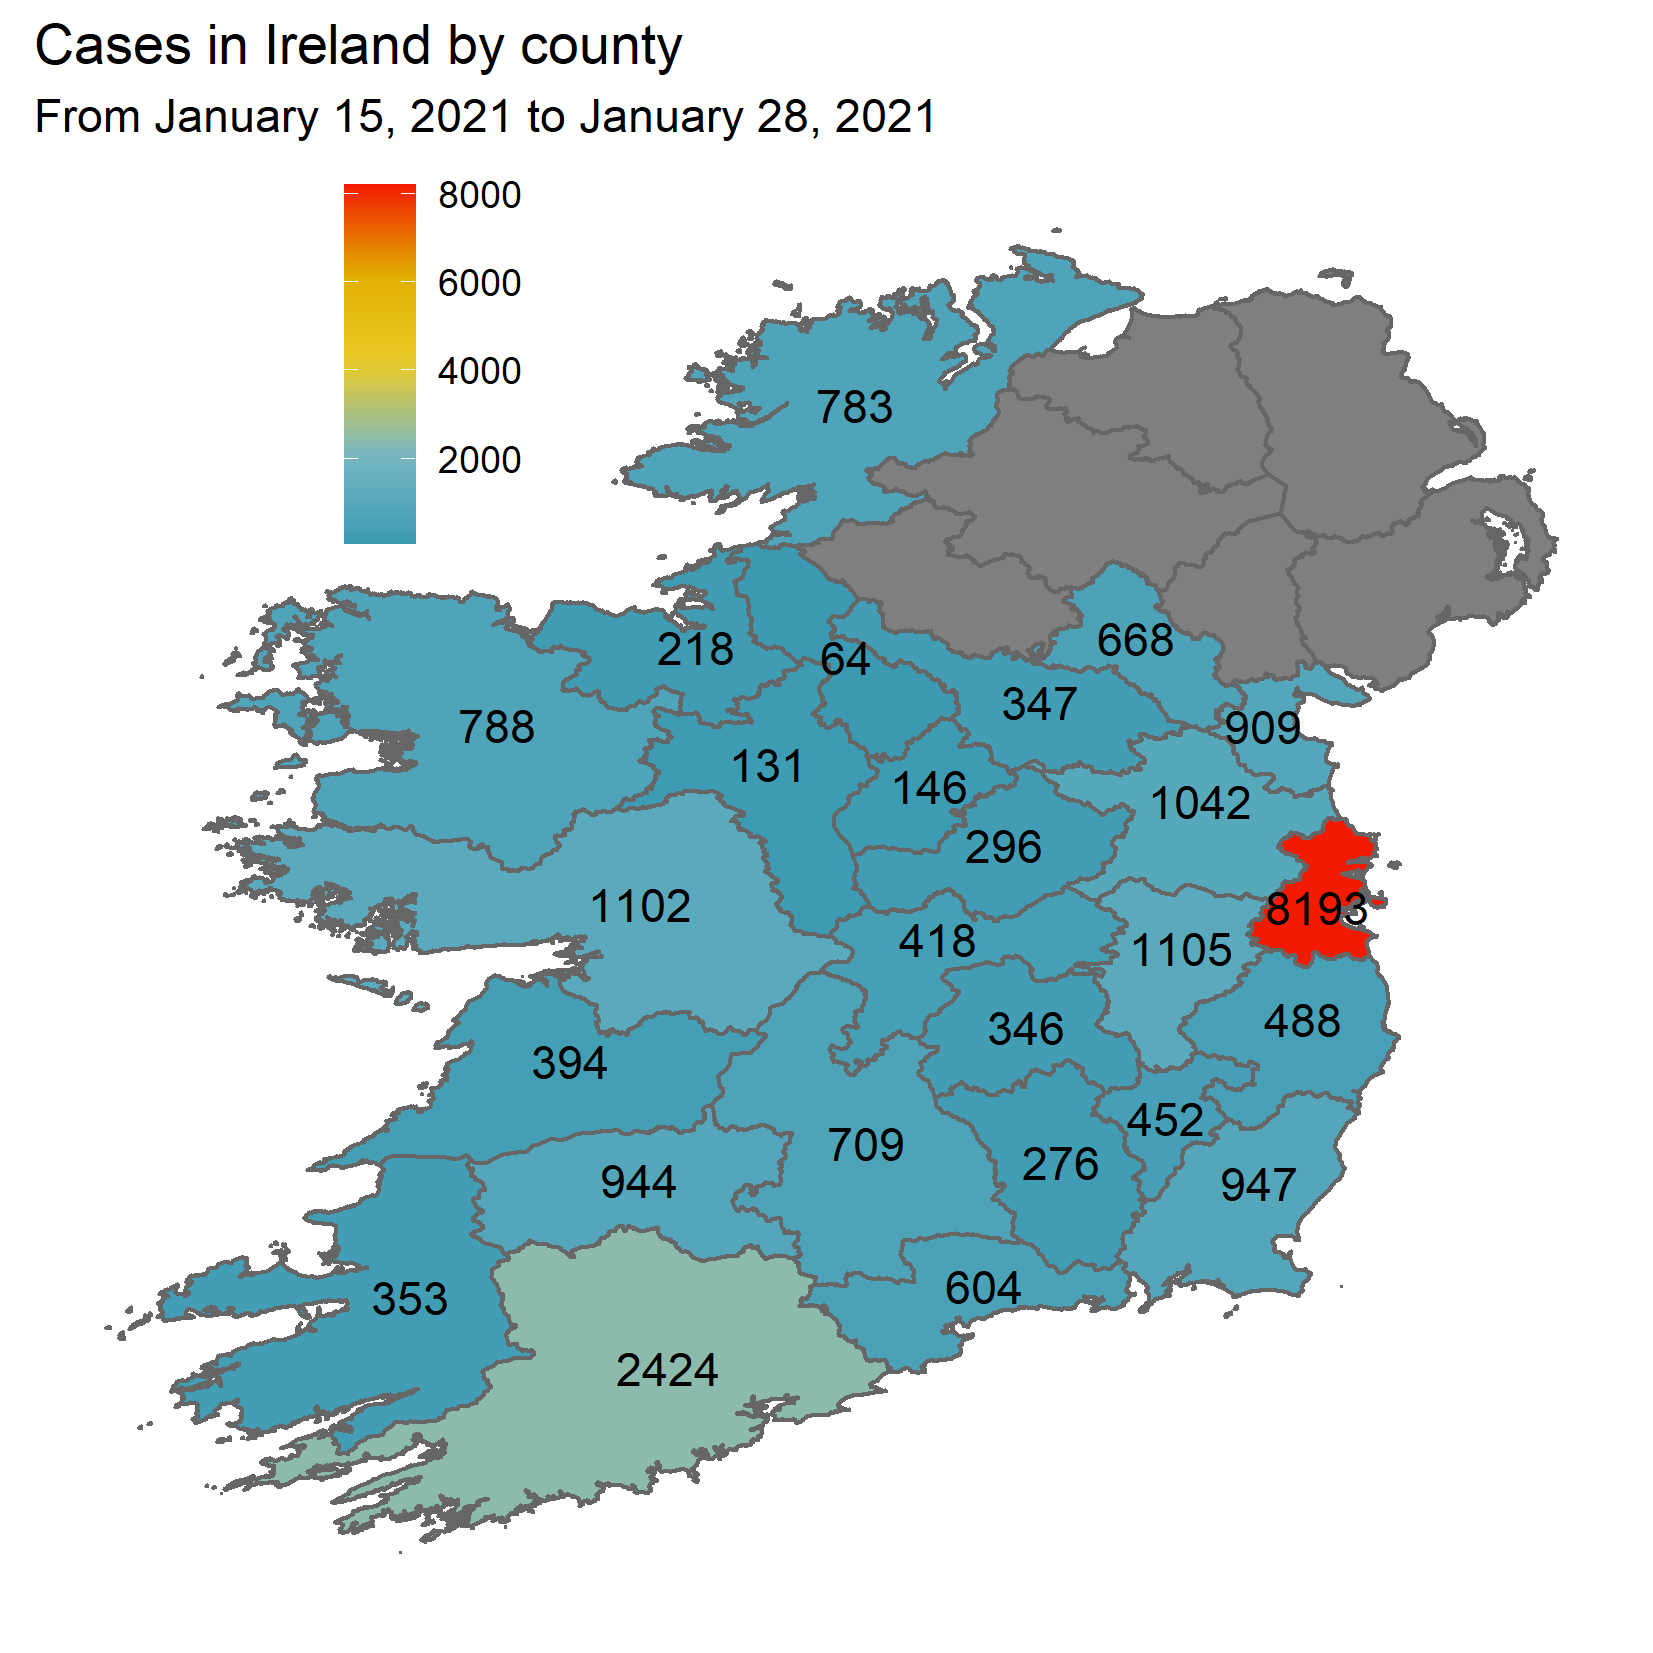
\includegraphics[width=0.9\textwidth]{county-fourteendaycases.png}


This project is based on the work in \cite{grigor20}, where I attempt to  reconstruct the recurrence relation to model the pandemic. This largely mathematical model (based on practical assumptions), but of course does not fit well in the long run. It is efficient at explaining singular phases of the pandemic, and calculating the infamous $R_0$ number, defined below, from \cite{epid08}. 

\begin{ndefinition} 
The number $R_0$ is called
the \textit{basic reproduction number} and is unquestionably the most important quantity to consider when analyzing any epidemic model for an infectious disease. Each infective individual can be expected to infect $R_0$ individuals. 
\end{ndefinition}

